\section{Mesures de clustering}
\label{sec:clustering}
% =====================================================================

\subsection{Sous-volumes et estimateur}

Chaque boîte de $2\,h^{-1}$Gpc est divisée en $4^3=64$ sous-volumes cubiques sans recouvrement de $500\Mpch$ (environ $62\,500$ galaxies chacun). Chaque sous-volume est traité comme un relevé indépendant à frontières ouvertes : les fonctions de corrélation sont mesurées avec l'estimateur de Landy--Szalay \cite{LandySzalay1993},
\begin{equation}
\xi(s,\mu) = \frac{D_1D_2 - D_1R - RD_2 + RR}{RR},
\end{equation}
en utilisant un catalogue uniforme de $5\times$ le nombre de galaxies pour décrire la géométrie (le même pour tous les sous-volumes, de sorte que $RR$ n'est calculé qu'une fois). Les comptages de paires sont calculés avec \texttt{pycorr}/\texttt{Corrfunc} \cite{Sinha2020} en 30 bins de $5\Mpch$ dans $s\in[0,150]\Mpch$ et 120 bins en $\mu\in[-1,1]$, avec $\mu$ défini par rapport à la ligne de visée fixe, et projetés sur les multipôles de Legendre $\ell=0,2,4$ (seuls $\ell=0,2$ sont utilisés dans les prévisions).

\subsection{Statistiques}

Pour chaque méthode $m\in\{$ASTRA, DS$\}$, population $p\in\{$aléatoire, galaxie$\}$ et quartile Q$_i$, nous mesurons la corrélation croisée quartile--galaxie $\xi^{\rm QG}_{i,\ell}(s)$, entre les points de Q$_i$ et toutes les galaxies, et l'auto-corrélation du quartile $\xi^{\rm QQ}_{i,\ell}(s)$, ainsi que la fonction de corrélation à deux points des galaxies $\xi^{\rm GG}_\ell(s)$ (2PCF) : 33 statistiques par catalogue. Pour les quartiles aléatoires, $\xi^{\rm QG}$ et $\xi^{\rm QQ}$ sont les analogues des fonctions de corrélation croisée et d'auto-corrélation du density split \cite{Paillas2023}. Pour les quartiles de galaxies, qui partitionnent les galaxies en quatre ensembles égaux, la moyenne des quatre corrélations croisées quartile--galaxie est la 2PCF : les quartiles décomposent la 2PCF par environnement.

\subsection{Résultats sur la cosmologie fiducielle}

La Figure~\ref{fig:multipoles} compare les quartiles extrêmes des deux méthodes, et les Figures~\ref{fig:mp_astra} et~\ref{fig:mp_ds} montrent les quatre quartiles de chaque méthode dans la disposition des analyses de density split \cite{Paillas2023} ; les quartiles de galaxies sont montrés dans la Figure~\ref{fig:multipoles_gal}.

Les deux méthodes produisent des signaux qualitativement identiques. La corrélation croisée Q1--galaxie est négative aux petites séparations, le profil des galaxies autour des régions sous-denses, et la corrélation croisée Q4--galaxie est positive et au-dessus de la 2PCF des galaxies, le profil autour des régions surdenses. Les auto-corrélations des quartiles extrêmes sont fortement amplifiées par rapport à la 2PCF. Les quadrupôles ont des signes opposés pour Q1 et Q4 : autour des régions sous-denses, les vitesses particulières pointent vers l'extérieur et étirent le profil du vide le long de la ligne de visée, alors qu'autour des régions surdenses la chute gravitationnelle le comprime. Les quartiles intermédiaires Q2 et Q3 ont de faibles corrélations croisées de signes opposés, proches du champ moyen, et des auto-corrélations 5 à 6 fois inférieures à celles des quartiles extrêmes.

Les signaux ASTRA sont systématiquement plus faibles, d'un facteur $\sim1.6$ au pic des corrélations croisées Q1 et Q4 ($s^2\xi_0\simeq-90$ et $+90\,h^{-2}{\rm Mpc}^2$, contre $-145$ et $+145$ pour le density split). Cela est cohérent avec le mélange partiel des quartiles : ASTRA s'appuie sur $\sim15$ voisins par point, ce qui dilue le contraste entre environnements. Pour le density split, les auto-corrélations Q1 et Q4 sont presque égales, alors que pour ASTRA l'auto-corrélation Q1 culmine 40\% au-dessus de celle de Q4 : le quartile sous-dense d'ASTRA est relativement plus corrélé avec lui-même, un premier signe que ses auto-corrélations portent une information distincte. La question pertinente n'est pas l'amplitude du signal mais son contenu en information rapporté à son bruit, que nous abordons avec les prévisions.

\begin{figure*}[!tp]
\centering
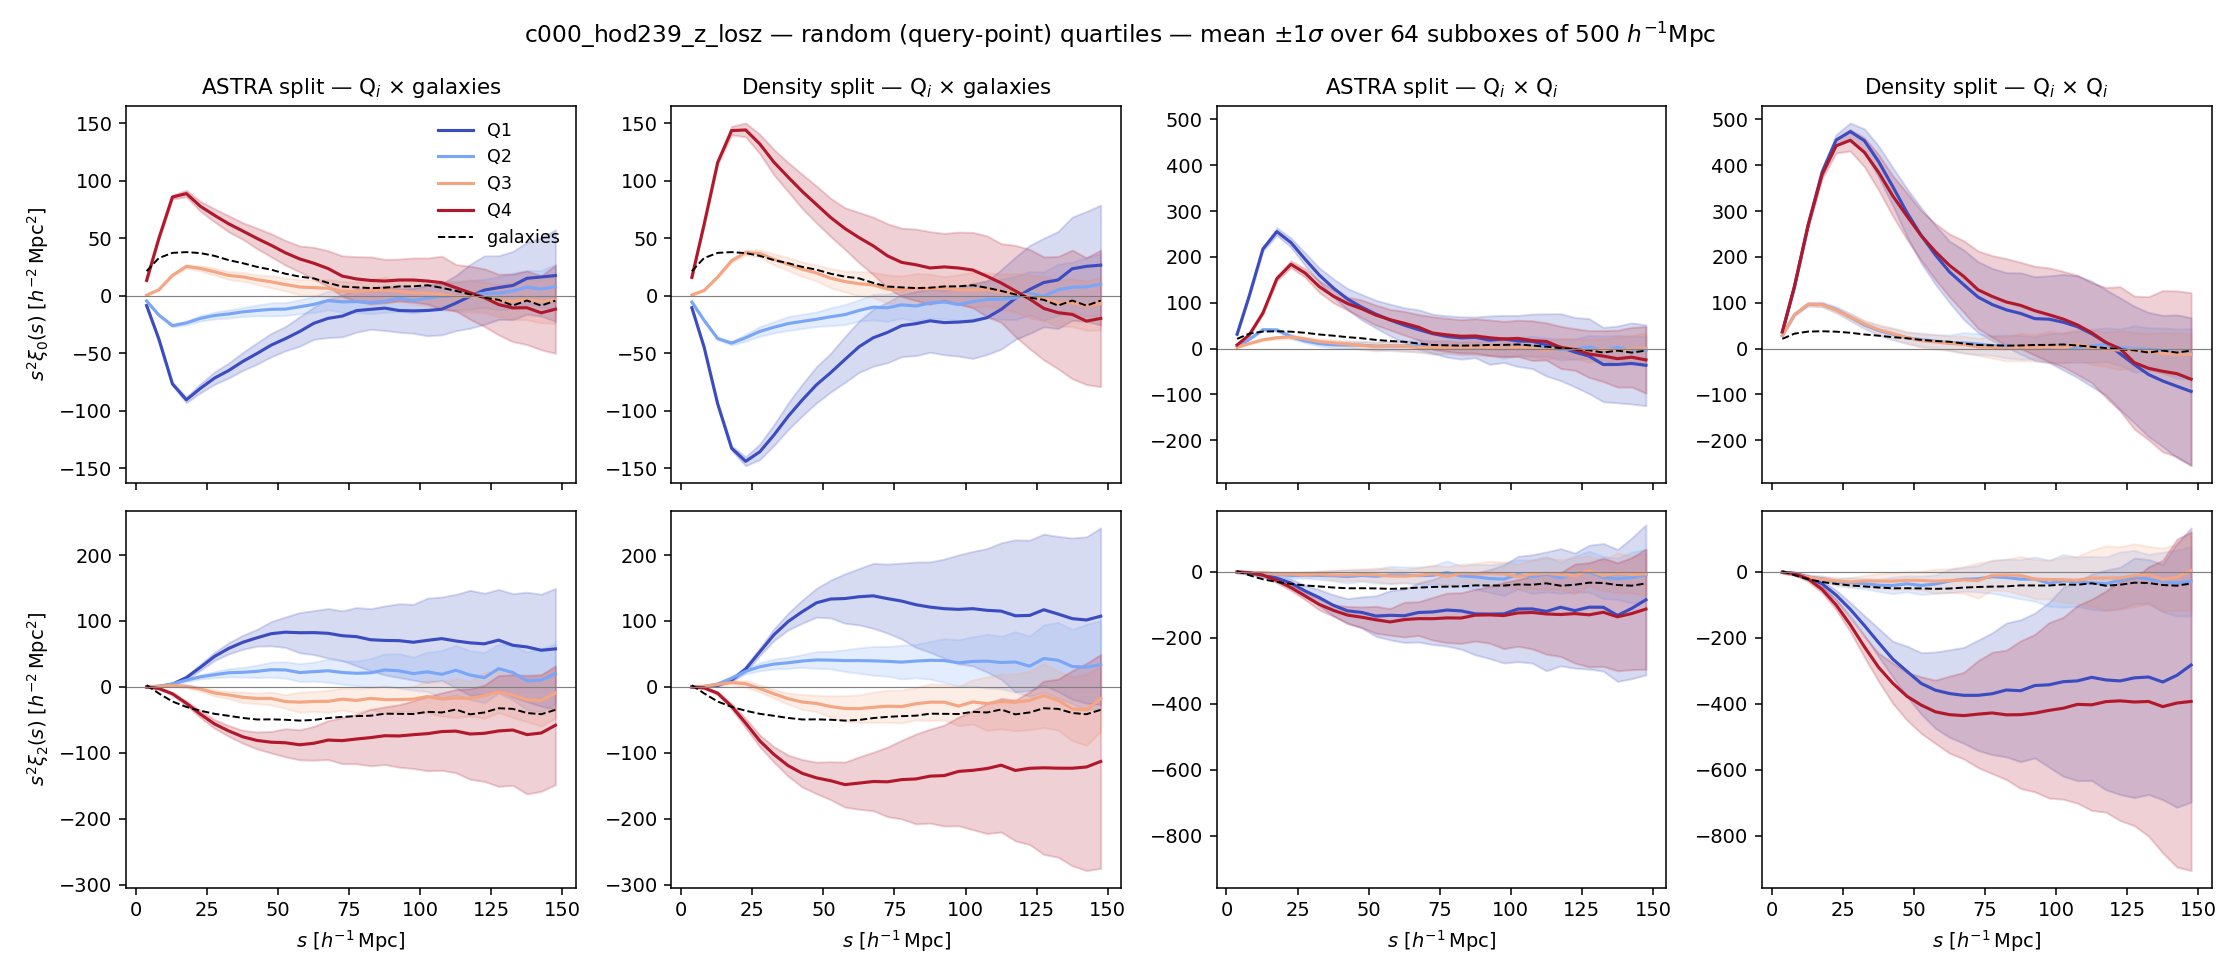
\includegraphics[width=\textwidth]{v2_multipoles_rand.png}
\caption{Monopôle (haut) et quadrupôle (bas) des statistiques des quartiles aléatoires sur le catalogue fiduciel, pour l'ASTRA split et le density split : corrélations croisées quartile--galaxie (deux colonnes de gauche) et auto-corrélations des quartiles (deux colonnes de droite), de Q1 (bleu) à Q4 (rouge) ; tirets : 2PCF des galaxies. Moyenne et dispersion à $1\sigma$ sur les 64 sous-volumes de $(500\Mpch)^3$ ; les panneaux d'une même statistique partagent la même échelle.}
\label{fig:multipoles}
\end{figure*}

\begin{figure}[!htbp]
\centering
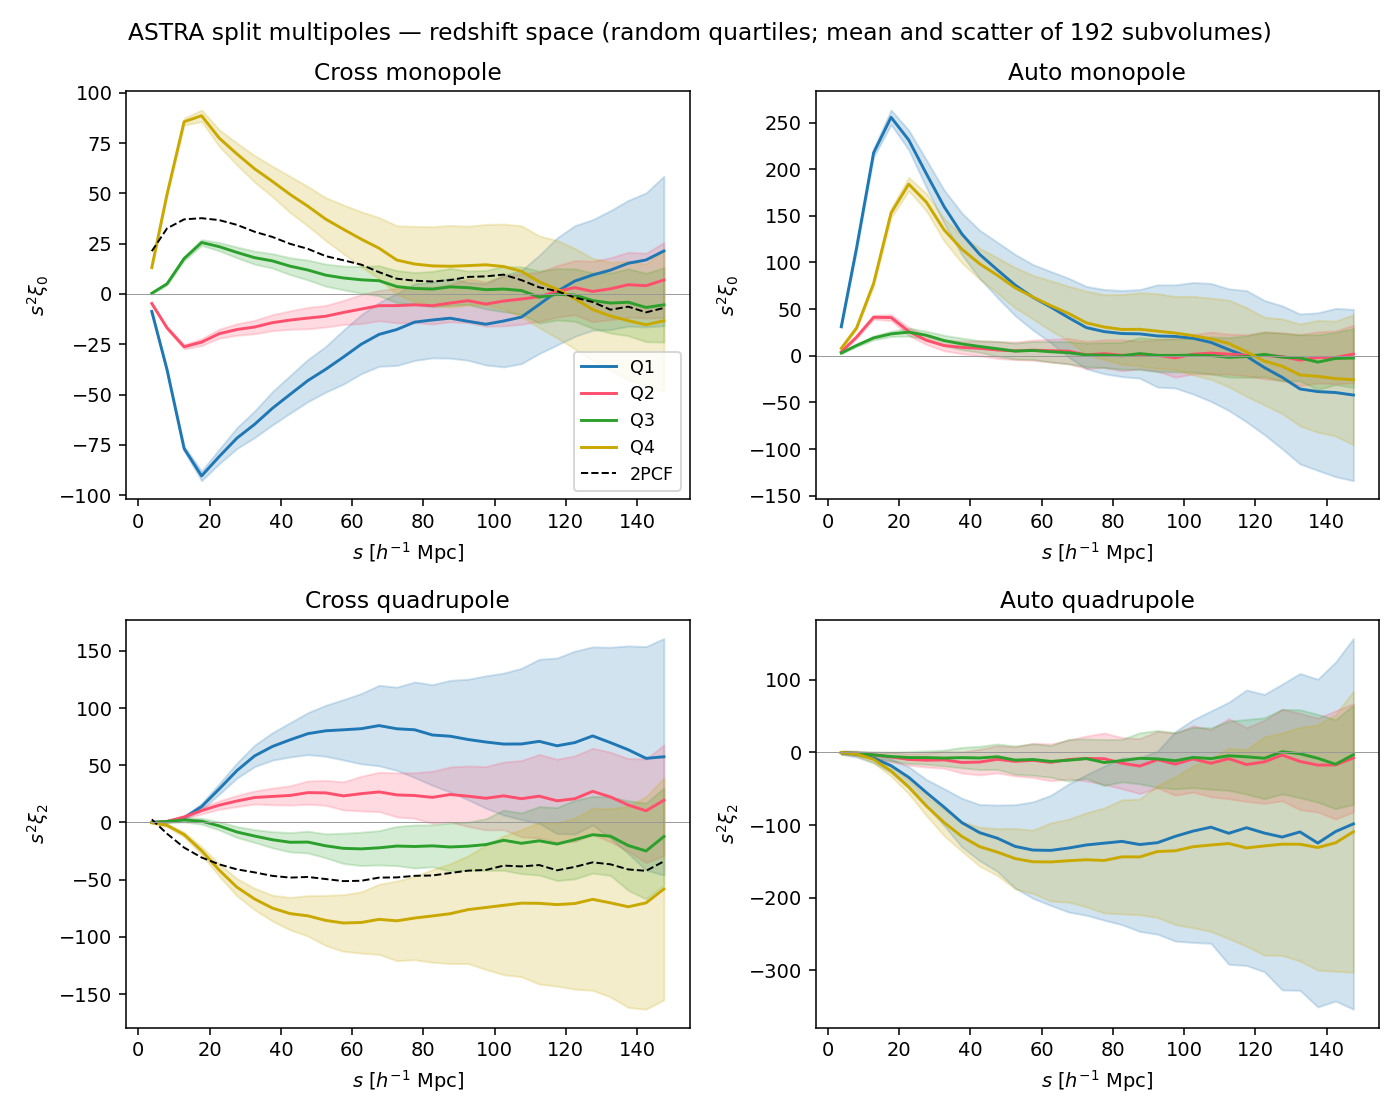
\includegraphics[width=\linewidth]{v1style_multipoles_astra.png}
\caption{ASTRA split : monopôle et quadrupôle des corrélations croisées quartile--galaxie (gauche) et des auto-corrélations des quartiles (droite) pour les quatre quartiles aléatoires ; tirets : 2PCF des galaxies. Moyenne et dispersion de 192 sous-volumes du catalogue fiduciel.}
\label{fig:mp_astra}
\end{figure}

\begin{figure}[!htbp]
\centering
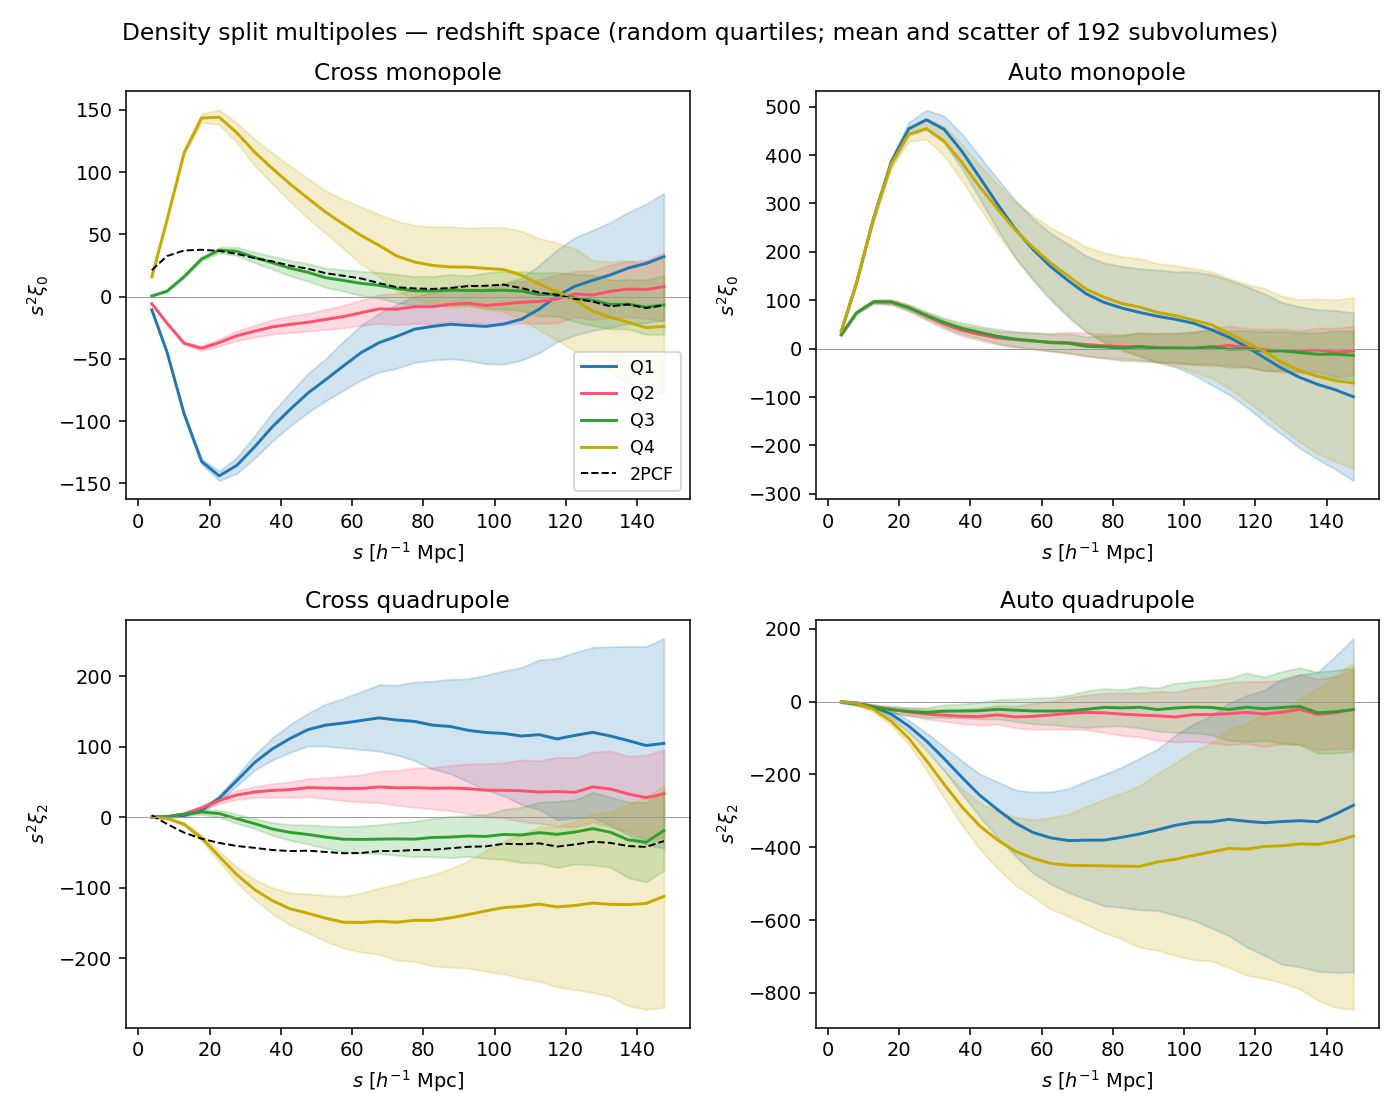
\includegraphics[width=\linewidth]{v1style_multipoles_ds.png}
\caption{Identique à la Figure~\ref{fig:mp_astra} pour le density split.}
\label{fig:mp_ds}
\end{figure}

\begin{figure*}[!tp]
\centering
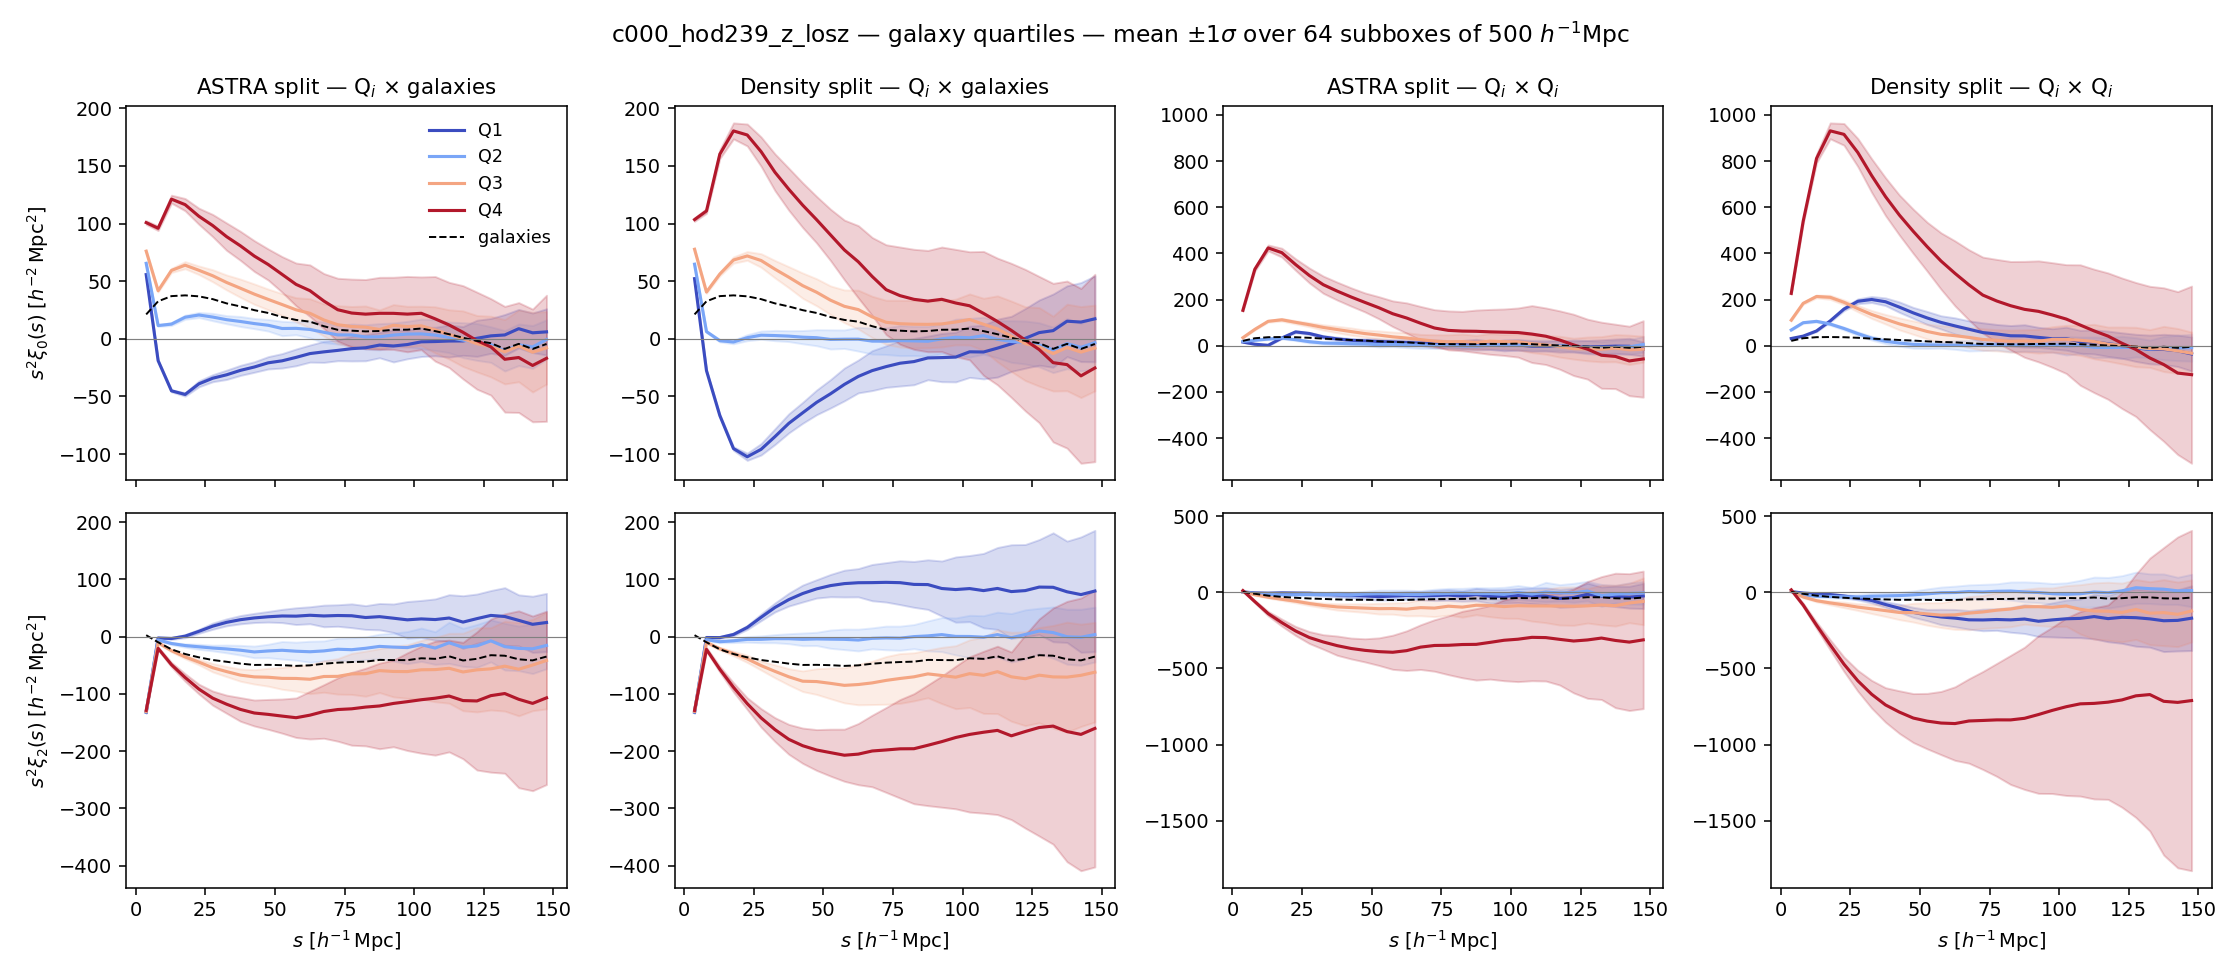
\includegraphics[width=\textwidth]{v2_multipoles_gal.png}
\caption{Identique à la Figure~\ref{fig:multipoles} pour les quartiles de galaxies.}
\label{fig:multipoles_gal}
\end{figure*}

\subsection{Espace réel et espace des redshifts}

Pour isoler l'effet des RSD, nous avons aussi mesuré le catalogue fiduciel (et les huit catalogues des paires de dérivées) dans l'espace réel, les environnements étant alors définis à partir des positions dans l'espace réel (r-split) au lieu de celles de l'espace des redshifts (z-split), selon les trois lignes de visée. La Figure~\ref{fig:realz} compare les deux. Les RSD augmentent les monopôles à $20$--$60\Mpch$ d'un facteur 1.6 pour la 2PCF des galaxies et de 1.3--1.5 pour les corrélations croisées Q1 et Q4 des deux méthodes, et créent des quadrupôles absents dans l'espace réel : positifs autour des régions sous-denses (flux sortants) et négatifs autour des régions surdenses (chute gravitationnelle). En valeur absolue, les quadrupôles du density split sont 1.6 à 1.7 fois plus grands que ceux de l'ASTRA split, à l'image de leurs monopôles plus grands ; relativement au monopôle, cependant, le quadrupôle ASTRA est le plus grand ($|\xi_2|/|\xi_0|\simeq0.8$ pour ASTRA contre $0.6$ pour le density split pour Q1, $1.0$ contre $0.8$ pour Q4, à $20$--$60\Mpch$) : les environnements ASTRA sont moins contrastés mais leur anisotropie dans l'espace des redshifts est relativement plus forte. Les environnements de l'espace réel ne sont pas observables, donc toutes les prévisions utilisent le z-split ; les mesures dans l'espace réel sont conservées comme diagnostic. (Une première version de ce travail utilisait l'espace réel comme « vérité » pour quantifier des « biais systématiques » des prévisions dans l'espace des redshifts ; comme les mesures et l'émulateur sont tous deux dans l'espace des redshifts, cette comparaison ne décrit pas un biais de l'analyse, et la systématique pertinente, l'erreur de l'émulateur, est incluse dans la covariance.)

\begin{figure*}[!tp]
\centering
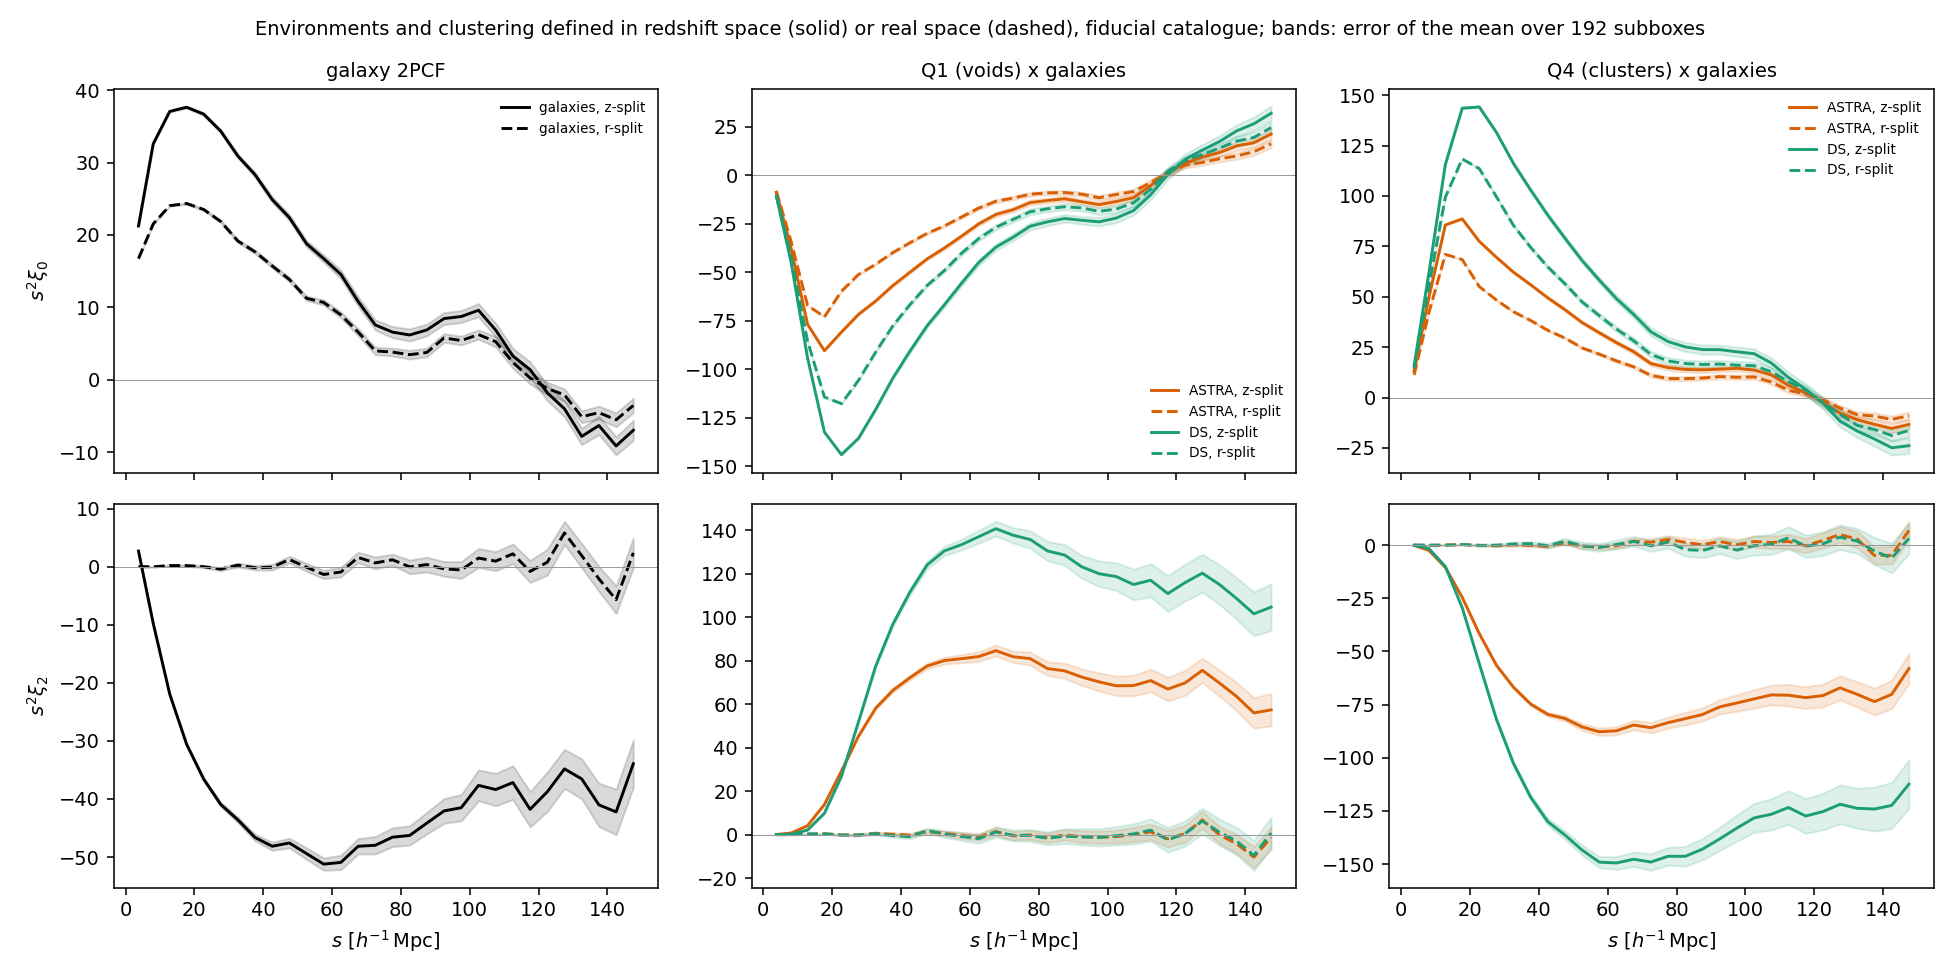
\includegraphics[width=\textwidth]{v2_real_vs_redshift.png}
\caption{Environnements et clustering définis dans l'espace des redshifts (trait plein) ou dans l'espace réel (tirets) pour le catalogue fiduciel : 2PCF des galaxies (gauche), corrélations croisées des quartiles aléatoires Q1 (centre) et Q4 (droite) de l'ASTRA split (orange) et du density split (vert). Haut : monopôle, bas : quadrupôle. Bandes : erreur sur la moyenne de $3\times64$ sous-volumes.}
\label{fig:realz}
\end{figure*}

